\documentclass{book}

\usepackage{fontspec}
\usepackage{polyglossia}
%\setmainfont[Mapping=tex-text]{CMU Serif}
\setmainlanguage{russian}
\setotherlanguage{english}
% XeLaTeX can use any font installed in your system fonts folder
\newfontfamily\russianfont[Script=Cyrillic]{CMU Serif}
%\newfontfamily\russianfont[Script=Cyrillic]{Droid Serif}

\usepackage{etex}
\usepackage{savesym}
\usepackage{amssymb, amsmath,amsthm,amscd}
%\savesymbol{lrcorner}
\usepackage{txfonts}
\savesymbol{lrcorner}\savesymbol{llcorner}\savesymbol{urcorner}\savesymbol{ulcorner}
%\usepackage{marvosym}
\usepackage{wasysym}
\savesymbol{Sun}\savesymbol{Mercury}\savesymbol{Venus}\savesymbol{Earth}\savesymbol{Mars}\savesymbol{Jupiter}\savesymbol{Saturn}\savesymbol{Uranus}\savesymbol{Neptune}\savesymbol{Pluto}\savesymbol{leftmoon}\savesymbol{rightmoon}\savesymbol{fullmoon}\savesymbol{newmoon}\savesymbol{Aries}\savesymbol{Taurus}\savesymbol{Gemini}\savesymbol{Leo}\savesymbol{Libra}\savesymbol{Scorpio}\savesymbol{diameter}
\usepackage{mathabx}
%\usepackage{stmaryrd}
\usepackage{setspace}
\usepackage{chngcntr}
\usepackage[tt]{titlepic}
\usepackage{enumerate,makecell}
\usepackage{makeidx,tabularx,dashbox}
\usepackage[usenames,dvipsnames]{xcolor}
\usepackage[bookmarks=true,colorlinks=true, linkcolor=MidnightBlue, citecolor=cyan]{hyperref}
\usepackage{lmodern}
\usepackage{graphicx,float}
\usepackage{multirow}
\usepackage{geometry}
\newgeometry{left=1.6in,right=1.6in,top=1.4in,bottom=1.4in}
\restoresymbol{txfonts}{lrcorner}\restoresymbol{txfonts}{llcorner}\restoresymbol{txfonts}{urcorner}\restoresymbol{txfonts}{ulcorner}

\usepackage{color}
\usepackage[all,poly,color,matrix,arrow]{xy}
\makeindex

%\usepackage{showkeys}

\newcommand{\comment}[1]{}

\newcommand{\longnote}[2][4.9in]{\fcolorbox{black}{yellow}{\parbox{#1}{\color{black} #2}}}
\newcommand{\shortnote}[1]{\fcolorbox{black}{yellow}{\color{black} #1}}
\newcommand{\start}[1]{\shortnote{Start here: #1.}}
\newcommand{\q}[1]{\begin{question}#1\end{question}}
\newcommand{\g}[1]{\begin{guess}#1\end{guess}}
\newcommand{\cfbox}[2]{
    \colorlet{currentcolor}{.}
    {\color{#1}
    \fbox{\color{currentcolor}#2}}
}

\def\tn{\textnormal}
\def\mf{\mathfrak}
\def\mc{\mathcal}
\newcommand{\qt}[1]{\tn{``}#1\tn{"}}

\def\ZZ{{\mathbb Z}}
\def\QQ{{\mathbb Q}}
\def\RR{{\mathbb R}}
\def\CC{{\mathbb C}}
\def\AA{{\mathbb A}}
\def\PP{{\mathbb P}}
\def\NN{{\mathbb N}}


\def\Hom{\tn{Hom}}
\def\Path{\tn{Path}}
\def\Paths{\tn{Paths}}
\def\List{\tn{List}}
\def\Aut{\tn{Aut}}
\def\im{\tn{im}}
\def\Fun{\tn{Fun}}
\def\Ob{\tn{Ob}}
\def\Skel{\tn{Skel}}
\def\Op{\tn{Open}}
\def\PK{\tn{PK}}
\def\FK{\tn{FK}}
\def\SEL*{\tn{SEL*}}
\def\Res{\tn{Res}}
\def\hsp{\hspace{.3in}}
\newcommand{\hsps}[1]{{\hspace{2mm} #1\hspace{2mm}}}
\newcommand{\tin}[1]{\text{\tiny #1}}

\def\singleton{\{\smiley\}}
\newcommand{\boxtitle}[1]{\begin{center}#1\end{center}\vspace{-.1in}}
\newcommand{\singlefun}[1]{\star^{#1}}
\newcommand{\pullb}[1]{\Delta_{#1}}
\newcommand{\lpush}[1]{\Sigma_{#1}}
\newcommand{\rpush}[1]{\Pi_{#1}}
\def\lcone{^\triangleleft}
\def\rcone{^\triangleright}
\def\to{\rightarrow}
\def\from{\leftarrow}
\def\down{\downarrrow}
\def\Down{\Downarrow}
\def\taking{\colon}
\def\inj{\hookrightarrow}
\def\surj{\twoheadrightarrow}
\def\too{\longrightarrow}
\newcommand{\xyright}[1]{\xymatrix{~\ar[r]#1&}}
\newcommand{\xydown}[1]{\xymatrix{~\ar[d]#1\\~}}
\newcommand{\xydoown}[1]{\xymatrix{~\ar[ddd]#1\\\parbox{0in}{~}\\\parbox{0in}{~}\\~}}
\def\fromm{\longleftarrow}
\def\tooo{\longlongrightarrow}
\def\tto{\rightrightarrows}
\def\ttto{\equiv\!\!>}
\def\ss{\subseteq}
\def\superset{\supseteq}
\def\iso{\cong}
\def\down{\downarrow}
\def\|{{\;|\;}}
\def\m1{{-1}}
\def\op{^\tn{op}}
\def\loc{\tn{loc}}
\def\la{\langle}
\def\ra{\rangle}
\def\wt{\widetilde}
\def\wh{\widehat}
\def\we{\simeq}
\def\ol{\overline}
\def\ul{\underline}
\def\plpl{+\!\!+\hspace{1pt}}
\def\acts{\lefttorightarrow}
\def\actsRight{\righttoleftarrow}
\def\vect{\overrightarrow}
\def\qeq{\mathop{=}^?}
\def\del{\partial\,}

\def\rr{\raggedright}

%\newcommand{\LMO}[1]{\bullet^{#1}}
%\newcommand{\LTO}[1]{\bullet^{\tn{#1}}}
\newcommand{\LMO}[1]{\stackrel{#1}{\bullet}}
\newcommand{\LTO}[1]{\stackrel{\tt{#1}}{\bullet}}
\newcommand{\LA}[2]{\ar[#1]^-{\tn {#2}}}
\newcommand{\LAL}[2]{\ar[#1]_-{\tn {#2}}}
\newcommand{\obox}[3]{\stackrel{#1}{\fbox{\parbox{#2}{#3}}}}
\newcommand{\labox}[2]{\obox{#1}{1.6in}{#2}}
\newcommand{\mebox}[2]{\obox{#1}{1in}{#2}}
\newcommand{\smbox}[2]{\stackrel{#1}{\fbox{#2}}}
\newcommand{\fakebox}[1]{\tn{$\ulcorner$#1$\urcorner$}}
\newcommand{\sq}[4]{\xymatrix{#1\ar[r]\ar[d]&#2\ar[d]\\#3\ar[r]&#4}}
\newcommand{\namecat}[1]{\begin{center}$#1:=$\end{center}}

\def\monOb{\blacktriangle}

\def\ullimit{\ar@{}[rd]|(.3)*+{\lrcorner}}
\def\urlimit{\ar@{}[ld]|(.3)*+{\llcorner}}
\def\lllimit{\ar@{}[ru]|(.3)*+{\urcorner}}
\def\lrlimit{\ar@{}[lu]|(.3)*+{\ulcorner}}
\def\ulhlimit{\ar@{}[rd]|(.3)*+{\diamond}}
\def\urhlimit{\ar@{}[ld]|(.3)*+{\diamond}}
\def\llhlimit{\ar@{}[ru]|(.3)*+{\diamond}}
\def\lrhlimit{\ar@{}[lu]|(.3)*+{\diamond}}
\newcommand{\clabel}[1]{\ar@{}[rd]|(.5)*+{#1}}
\newcommand{\TriRight}[7]{\xymatrix{#1\ar[dr]_{#2}\ar[rr]^{#3}&&#4\ar[dl]^{#5}\\&#6\ar@{}[u] |{\Longrightarrow}\ar@{}[u]|>>>>{#7}}}
\newcommand{\TriLeft}[7]{\xymatrix{#1\ar[dr]_{#2}\ar[rr]^{#3}&&#4\ar[dl]^{#5}\\&#6\ar@{}[u] |{\Longleftarrow}\ar@{}[u]|>>>>{#7}}}
\newcommand{\TriIso}[7]{\xymatrix{#1\ar[dr]_{#2}\ar[rr]^{#3}&&#4\ar[dl]^{#5}\\&#6\ar@{}[u] |{\Longleftrightarrow}\ar@{}[u]|>>>>{#7}}}


\newcommand{\arr}[1]{\ar@<.5ex>[#1]\ar@<-.5ex>[#1]}
\newcommand{\arrr}[1]{\ar@<.7ex>[#1]\ar@<0ex>[#1]\ar@<-.7ex>[#1]}
\newcommand{\arrrr}[1]{\ar@<.9ex>[#1]\ar@<.3ex>[#1]\ar@<-.3ex>[#1]\ar@<-.9ex>[#1]}
\newcommand{\arrrrr}[1]{\ar@<1ex>[#1]\ar@<.5ex>[#1]\ar[#1]\ar@<-.5ex>[#1]\ar@<-1ex>[#1]}

\newcommand{\To}[1]{\xrightarrow{#1}}
\newcommand{\Too}[1]{\xrightarrow{\ \ #1\ \ }}
\newcommand{\From}[1]{\xleftarrow{#1}}
\newcommand{\Fromm}[1]{\xleftarrow{\ \ #1\ \ }}

\newcommand{\Adjoint}[4]{\xymatrix@1{#2 \ar@<.5ex>[r]^-{#1} & #3 \ar@<.5ex>[l]^-{#4}}}
\newcommand{\adjoint}[4]{\xymatrix{#1\taking #2\ar@<.5ex>[r]& #3\hspace{1pt}:\hspace{-2pt} #4\ar@<.5ex>[l]}}

\newcommand{\prodmap}[2]{\la#1,#2\ra}
\newcommand{\pb}[3]{\prodmap{#1}{#1}_{#3}}
\newcommand{\coprodmap}[2]{{\left\{\parbox{.1in}{#1\\#2}\right.}}
\newcommand{\po}[3]{\coprodmap{#1}{#2}}

\def\id{\tn{id}}
\def\ids{\tn{ids}}
\def\Top{{\bf Top}}
\def\Cat{{\bf Cat}}
\def\Oprd{{\bf Oprd}}
\def\Str{{\bf Str}}
\def\Mon{{\bf Mon}}
\def\Grp{{\bf Grp}}
\def\Grph{{\bf Grph}}
\def\Type{{\bf Type}}
\def\Supp{{\bf Supp}}
\def\Dist{{\bf Dist}}
\def\Vect{{\bf Vect}}
\def\Kls{{\bf Kls}}
\def\Prop{{\bf Prop}}
\def\FLin{{\bf FLin}}
\def\Set{{\bf Set}}
\def\Sets{{\bf Sets}}
\def\PrO{{\bf PrO}}
\def\Star{{\bf Star}}
\def\Cob{{\bf Cob}}
\def\Qry{{\bf Qry}}
\def\set{{\text \textendash}{\bf Set}}
\def\sSet{{\bf sSet}}
\def\sSets{{\bf sSets}}
\def\Grpd{{\bf Grpd}}
\def\Pre{{\bf Pre}}
\def\Shv{{\bf Shv}}
\def\Rings{{\bf Rings}}
\def\bD{{\bf \Delta}}
\def\dispInt{\parbox{.1in}{$\int$}}
\def\bhline{\Xhline{2\arrayrulewidth}}
\def\bbhline{\Xhline{2.5\arrayrulewidth}}
\def\bbbhline{\Xhline{3\arrayrulewidth}}


\def\colim{\mathop{\tn{colim}}}
\def\hocolim{\mathop{\tn{hocolim}}}

\def\mcA{\mc{A}}
\def\mcB{\mc{B}}
\def\mcC{\mc{C}}
\def\mcD{\mc{D}}
\def\mcE{\mc{E}}
\def\mcF{\mc{F}}
\def\mcG{\mc{G}}
\def\mcH{\mc{H}}
\def\mcI{\mc{I}}
\def\mcJ{\mc{J}}
\def\mcK{\mc{K}}
\def\mcL{\mc{L}}
\def\mcM{\mc{M}}
\def\mcN{\mc{N}}
\def\mcO{\mc{O}}
\def\mcP{\mc{P}}
\def\mcQ{\mc{Q}}
\def\mcR{\mc{R}}
\def\mcS{\mc{S}}
\def\mcT{\mc{T}}
\def\mcU{\mc{U}}
\def\mcV{\mc{V}}
\def\mcW{\mc{W}}
\def\mcX{\mc{X}}
\def\mcY{\mc{Y}}
\def\mcZ{\mc{Z}}

\def\undsc{\rule{2mm}{0.4pt}}
\def\Loop{{\mcL oop}}
\def\LoopSchema{{\parbox{.5in}{\fbox{\xymatrix{\LMO{s}\ar@(l,u)[]^f}}}}}

\newtheorem{theorem}[subsubsection]{Theorem}
\newtheorem{lemma}[subsubsection]{Lemma}
\newtheorem{proposition}[subsubsection]{Proposition}
\newtheorem{corollary}[subsubsection]{Corollary}
\newtheorem{fact}[subsubsection]{Fact}

\theoremstyle{remark}
\newtheorem{remark}[subsubsection]{Remark}
\newtheorem{example}[subsubsection]{Example}
\newtheorem{warning}[subsubsection]{Warning}
\newtheorem{question}[subsubsection]{Question}
\newtheorem{guess}[subsubsection]{Guess}
\newtheorem{answer}[subsubsection]{Answer}
\newtheorem{construction}[subsubsection]{Construction}
\newtheorem{rules}[subsubsection]{Rules of good practice}
\newtheorem{exc}[subsubsection]{Exercise}
\newenvironment{exercise}{\begin{exc}}{\hspace*{\fill}$\lozenge$\end{exc}}
\newtheorem{app}[subsubsection]{Application}
\newenvironment{application}{\begin{app}}{\hspace*{\fill}$\lozenge\lozenge$\end{app}}

%\newenvironment{exercise}{\addtocounter{theorem}{1}\vspace{.1in}\begin{sloppypar}\noindent{\em Exercise}\;\arabic{chapter}.\arabic{section}.\arabic{subsection}.\arabic{theorem}.}{\end{sloppypar}\vspace{.1in}}

\newenvironment{slogan}{\addtocounter{subsubsection}{1}\vspace{.1in}\begin{sloppypar}\noindent{\em Slogan}\;\arabic{chapter}.\arabic{section}.\arabic{subsection}.\arabic{subsubsection}. \begin{quote}``\slshape}{"\end{quote}\end{sloppypar}\vspace{.1in}}

%\newenvironment{application}{\addtocounter{subsubsection}{1}\vspace{.1in}\begin{sloppypar}\noindent{\em Application}\;\arabic{chapter}.\arabic{section}.\arabic{subsection}.\arabic{subsubsection}. \begin{quote}}{\end{quote}\end{sloppypar}\vspace{.1in}}
\makeatletter\let\c@figure\c@equation\makeatother%Aligns figure numbering and equation numbering.

\theoremstyle{definition}
\newtheorem{definition}[subsubsection]{Definition}
\newtheorem{notation}[subsubsection]{Notation}
\newtheorem{conjecture}[subsubsection]{Conjecture}
\newtheorem{postulate}[subsubsection]{Postulate}


%\newtheorem{theorem}{Theorem}[subsection]
%\newtheorem{lemma}[theorem]{Lemma}
%\newtheorem{proposition}[theorem]{Proposition}
%\newtheorem{corollary}[theorem]{Corollary}
%\newtheorem{fact}[theorem]{Fact}
%
%\theoremstyle{remark}
%\newtheorem{remark}[theorem]{Remark}
%\newtheorem{example}[theorem]{Example}
%\newtheorem{warning}[theorem]{Warning}
%\newtheorem{question}[theorem]{Question}
%\newtheorem{guess}[theorem]{Guess}
%\newtheorem{answer}[theorem]{Answer}
%\newtheorem{construction}[theorem]{Construction}
%\newtheorem{rules}[theorem]{Rules of good practice}
%\newtheorem{exc}[theorem]{Exercise}
%%\newenvironment{exercise}{\addtocounter{theorem}{1}\vspace{.1in}\begin{sloppypar}\noindent{\em Exercise}\;\arabic{chapter}.\arabic{section}.\arabic{subsection}.\arabic{theorem}.}{\end{sloppypar}\vspace{.1in}}
%\newenvironment{exercise}{\begin{exc}}{\hspace*{\fill}$\lozenge$\end{exc}}
%
%\theoremstyle{definition}
%\newtheorem{definition}[theorem]{Definition}
%\newtheorem{notation}[theorem]{Notation}
%\newtheorem{conjecture}[theorem]{Conjecture}
%\newtheorem{postulate}[theorem]{Postulate}

\def\Finm{{\bf Fin_{m}}}
\def\Prb{{\bf Prb}}
\def\Prbs{{\wt{\bf Prb}}}
\def\El{{\bf El}}
\def\Gr{{\bf Gr}}
\def\DT{{\bf DT}}
\def\DB{{\bf DB}}
\def\Tables{{\bf Tables}}
\def\Sch{{\bf Sch}}
\def\Fin{{\bf Fin}}
\def\P{{\bf P}}
\def\SC{{\bf SC}}
\def\ND{{\bf ND}}
\def\Poset{{\bf Poset}}


\newcommand{\MainCatLarge}[1]{
	\stackrel{#1}{
		\parbox{4.5in}{\fbox{\parbox{4.4in}{\begin{center}\underline{{\tt Employee} manager worksIn $\simeq$ {\tt Employee} worksIn}\hsp  \underline{{\tt Department} secretary worksIn $\simeq$ {\tt Department}}\end{center}~\\\\\\
			\xymatrix@=8pt{&\LTO{Employee}\ar@<.5ex>[rrrrr]^{\tn{worksIn}}\ar@(l,u)[]+<5pt,10pt>^{\tn{manager}}\ar[dddl]_{\tn{first}}\ar[dddr]^{\tn{last}}&&&&&\LTO{Department}\ar@<.5ex>[lllll]^{\tn{secretary}}\ar[ddd]^{\tn{name}}\\\\\\\LTO{FirstNameString}&&\LTO{LastNameString}&~&~&~&\LTO{DepartmentNameString}
			}
		}}}
	}
}
\def\GrIn{{\bf GrIn}}
\def\GrInSchema{\xymatrix{\LMO{Ar}\ar@<.5ex>[r]^{src}\ar@<-.5ex>[r]_{tgt}&\LMO{V\!e}}}
%\CompileMatrices
%\pdfoutput=1

\setcounter{secnumdepth}{3}
\setcounter{tocdepth}{1}

\def\sub{\begin{itemize}\item}
\def\sexc{\begin{enumerate}[a.)]\setlength{\itemsep}{.1cm}\setlength{\parskip}{.1cm}\item}
\def\next{\item}
\def\endsub{\end{itemize}}
\def\endsexc{\end{enumerate}}

%%%%%

\begin{document}
\begin{english}

\title{
  ~\\Category Theory for Scientists\\
  \begin{russian}Теория категорий для науки\end{russian}
}
\author{
  David I. Spivak\\
  \begin{russian}Дэвид И. Спивак\end{russian}
}
\titlepic{\vspace{1.3in}\dashbox{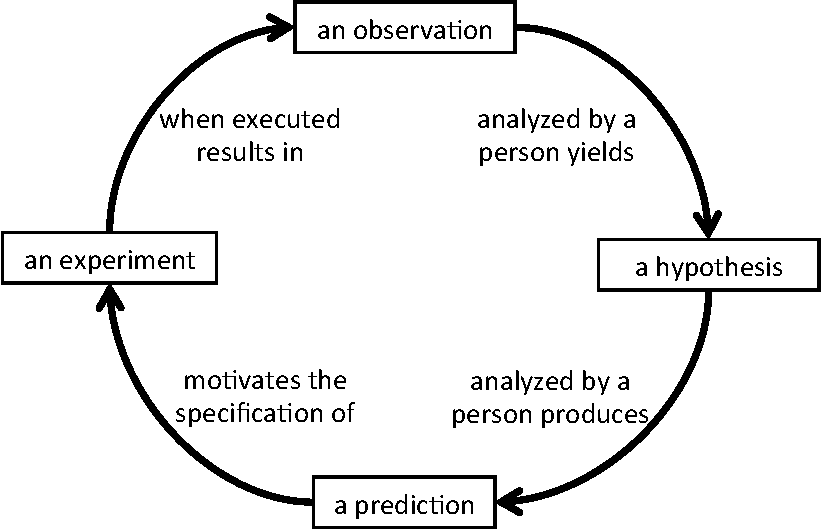
\includegraphics[width=.8\textwidth]{ScientificMethod}}\\\vspace{.3in}\Large How can mathematics make this diagram meaningful?%What does this diagram intend to communicate?
\normalsize}
\maketitle

\chapter*{Preface / Предисловие}

An early version of this book was put on line in February 2013 to serve as the textbook for my course \href{http://math.mit.edu/~dspivak/teaching/sp13/}{\text Category Theory for Scientists} taught in the spring semester of 2013 at MIT. During that semester, students provided me with hundreds of comments and questions, which led to a substantial improvement (and the addition of 50 pages) to the original document.

\begin{russian}Ранняя версия данной книги была представлена в феврале 2013 в качестве учебника для моего курса \href{http://math.mit.edu/~dspivak/teaching/sp13/}{\text Теория категорий для ученых}, который читался в весеннем семестре 2013 в MIT. В течение семестра студенты передали мне сотни комментариев и вопросов, которые привели к существенному улучшению исходного текста (и к добавлению 50 страниц).\end{russian}

In the summer of 2013 I signed a contract with the MIT Press to publish a new version of this work under the title {\em Category Theory for the Sciences}. Because I am committed to the open source development model I insisted that a version of this book, namely the one you are reading, remain freely available online. The MIT Press version will of course not be free.

\begin{russian}Летом 2013 я подписал контракт с MIT Press о публикации новой версии данной работы под заглавием {\em Теория категорий для наук}. Поскольку я являюсь приверженцем подхода открытого исходного кода, я настоял на том, что отдельная версия этой книги, а именно --- та, которую вы сейчас читаете, останется доступной бесплатно онлайн. \end{russian}

Other than the title, there are two main differences between the present version and the MIT Press version. The first difference is that I will do a full edit with the help of professional editors from the Press. The second difference is that I will write up solutions to the book's (approximately 280) exercises; some of these will be included in the published version, whereas the rest will be available by way of a password-protected page, accessible only to professors who teach the subject.

\begin{russian}Помимо заголовка, есть еще два основных различия данной версии и версии MIT Press. Первое различие состоит в том, что я проведу кардинальное редактирование при помощи профессиональных редакторов. Второе различие --- в том, что я напишу решения для упражнений этой книги (приблизительно 280); некоторые из них будут включены в опубликованную версию, тогда как остальные будут размещены на защищенной паролем странице, доступные только преподавателям, ведущим данный предмет. \end{russian}

\begin{russian}
\tableofcontents
\end{russian}

%%%%%%%% Chapter %%%%%%%%

\chapter{Introduction / Введение}

The title page of this book contains a graphic that we reproduce here.\\
\begin{russian}Титульная страница данной книги содержит рисунок, который мы воспроизводим ниже.\end{russian}
\begin{align}\label{dia:scientific method}
\dashbox{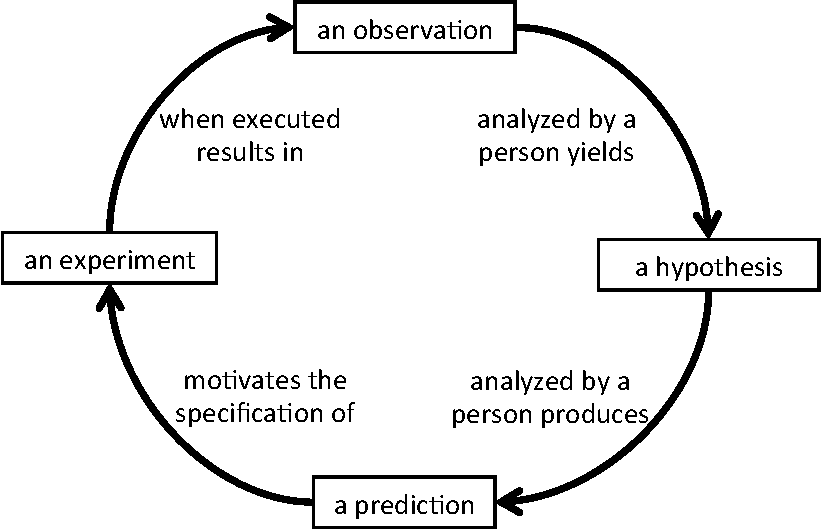
\includegraphics[width=.7\textwidth]{ScientificMethod}}
\end{align}
It is intended to evoke thoughts of the scientific method.\\
\begin{russian}Он призван наводить на мысли о научном методе.\end{russian} \begin{quote}
A hypothesis analyzed by a person produces a prediction, which motivates the specification of an experiment, which when executed results in an observation, which analyzed by a person yields a hypothesis.

\begin{russian}Гипотеза, выведенная человеком, приводит к предсказанию, которое мотивирует описание эксперимента, который, после выполнения, приводит к наблюдениям, которые, будучи проанализированы человеком, приводят к гипотезе.\end{russian}
\end{quote}
This sounds valid, and a good graphic can be exceptionally useful for leading a reader through the story that the author wishes to tell. \\
\begin{russian}Это похоже на истину; кроме того, хорошая картинка может быть исключительно полезна, чтобы провести читателя сквозь историю, которую автор желает поведать.\end{russian}

Interestingly, a graphic has the power to evoke feelings of understanding, without really meaning much. The same is true for text: it is possible to use a language such as English to express ideas that are never made rigorous or clear. When someone says ``I believe in free will," what does she believe in? We may all have some concept of what she's saying---something we can conceptually work with and discuss or argue about. But to what extent are we all discussing the same thing, the thing she intended to convey?

\begin{russian}Любопытный факт: картинка имеет способность вызывать ощущение понимания, не неся при этом особого смысла. То же верно и для слов: язык вроде английского способен выражать идеи, которые в принципе невозможно сделать строгими или ясными. Если некто заявляет "Я верю в свободу воли," то во что некто верит? Все мы можем иметь некоторые представления о том, что этот некто говорит --- такие, с которыми можно концептуально работать, рассуждать, аргументировать. Но до какой степени мы все будем обсуждать одну и ту же вещь, --- вещь, которую некто собирался сообщить? \end{russian}

Science is about agreement. When we supply a convincing argument, the result of this convincing is agreement. When, in an experiment, the observation matches the hypothesis---success!---that is agreement. When my methods make sense to you, that is agreement. When practice does not agree with theory, that is disagreement. Agreement is the good stuff in science; it's the high fives.

\begin{russian} Суть науки --- в согласии. Когда мы предлагаем убедительный аргумент,  результатом этой убедительности является согласие. Когда в ходе эксперимента наблюдения совпадают с гипотезой, --- вот удача! --- это согласие. Когда мои методы имеют смысл и для вас, это согласие. Когда же практика не соответствует теории, это несогласие. Согласие --- вот лучшая материя в науке; оно подобно рукопожатию. \end{russian}

But it is easy to think we're in agreement, when really we're not. Modeling our thoughts on heuristics and pictures may be convenient for quick travel down the road, but we're liable to miss our turnoff at the first mile. The danger is in mistaking our convenient conceptualizations for what's actually there. It is imperative that we have the ability at any time to ground out in reality. What does that mean?

\begin{russian} Однако легко попасть в ситуацию, когда мы думаем, будто согласны, но на самом деле это не так. Моделирования наших размышлений в эвристиках или картинках может быть удобно для быстрого движения напрямик, но нам самим придется нести ответственность, если мы пропустим нужный поворот на первой же миле. Опасность --- в ошибочном выборе слишком удобной концептуализации для того, что происходит в на самом деле. В любой момент необходимо иметь возможность привязаться к реальности. Что это означает? \end{russian}

Data. Hard evidence. The physical world. It is here that science touches down and heuristics evaporate. So let's look again at the diagram on the cover. It is intended to evoke an idea of how science is performed. Is there hard evidence and data to back this theory up? Can we set up an experiment to find out whether science is actually performed according to such a protocol? To do so we have to shake off the stupor evoked by the diagram and ask the question: ``what does this diagram intend to communicate?"

\begin{russian} Данные. Железные подтверждения. Физический мир. Именно здесь наука приземляется, и испаряются эвристики. Так что давайте взглянем на диаграмму на обложке еще раз. Она предназначена вызывать идею о том, как делают науку. Но имеются ли железные подтверждения и данные, стоящие за подобной теорией? Способны ли мы организовать эксперимент для проверки того, что науку делают именно в соответствии с подобным протоколом? Чтобы сделать это, мы должны сбросить ступор, вызванный диаграммой, и задаться вопросом: "Что эта диаграмма должна нам сообщать?" \end{russian}

In this course I will use a mathematical tool called {\em ologs}, or ontology logs, to give some structure to the kinds of ideas that are often communicated in pictures like the one on the cover. Each olog inherently offers a framework in which to record data about the subject. More precisely it encompasses a {\em database schema}, which means a system of interconnected tables that are initially empty but into which data can be entered. For example consider the olog below\\
\begin{russian}В этом курсе я буду использовать математический инструмент, называемый {\em ологами} или же онтологическими записями, чтобы придать некую структуру тем видам идей, о которых зачастую сообщается в картинках, подобных той, что изображена на обложке. Каждый олог по своей сути представляет собой конструкцию, в которой записаны данные о предмете обсуждения. Более точно, они отражают {\em схему базы данных}, что означает систему взаимосвязанных таблиц, которые вначале пусты, но в которые могут быть внесены данные. Для примера рассмотрим такой олог \end{russian}
$$\xymatrix{
\obox{}{.5in}{\begin{russian}масса\end{russian}}&&\obox{}{1.1in}{\begin{russian}объект массы \end{russian}$m$ \begin{russian}удерживаемый на высоте \end{russian}$h$ \begin{russian}над землей\end{russian}}\LAL{ll}{\footnotesize\begin{russian}имеет массу\end{russian}}\LA{rrdd}{\hspace{.4in}\parbox{1in}{\singlespace \footnotesize \begin{russian}при падении требуется определенное число секунд до ударения о землю\end{russian}}}\LAL{dd}{\parbox{.7in}{\singlespace\footnotesize\begin{russian}имеет высоту в метрах\end{russian}}}&&\\\\
&&\obox{}{1in}{\begin{russian}действительное число \end{russian} $h$}\ar@{}[uurr]|(.35){?}\ar[rr]_-{\sqrt{2h\div 9.8}}&\hspace{.3in}&\obox{}{.9in}{\begin{russian}действительное число \end{russian} }
}
$$
This olog represents a framework in which to record data about objects held above the ground, their mass, their height, and a comparison (the ?-mark in the middle) between the number of seconds till they hit the ground and a certain real-valued function of their height. We will discuss ologs in detail throughout this course.\\
\begin{russian}Данный олог представляет собой конструкцию, в которой для объектов, находящихся над поверхностью земли, записаны: их масса, их высота и соответствие (значок ? в середине) между числом секунд, за которое они достигают земли, с определенной действительнозначной функцией их высоты. Ологи мы детально обсудим по ходу этого курса. \end{russian}

The picture in (\ref{dia:scientific method}) looks like an olog, but it does not conform to the rules that we lay out for ologs in Section \ref{sec:ologs}. In an olog, every arrow is intended to represent a mathematical function. It is difficult to imagine a function that takes in predictions and outputs experiments, but such a function is necessary in order for the arrow\\
\begin{russian} Картинка "научного метода" (\ref{dia:scientific method}) выглядит как олог, но она не соответствует правилам, которые мы изложим в Разделе \ref{sec:ologs}. В ологе каждая стрелка должна представлять математическую функцию. Трудно вообразить функцию, которая принимала бы предсказания и выдавала в результате эксперименты, но такая функция была бы необходима, чтобы стрелка \end{russian}
$$\fbox{\begin{russian}предсказание\end{russian}}\To{\tn{\begin{russian}мотивирует спецификацию\end{russian}}}\fbox{\begin{russian}эксперимент\end{russian}}
$$
in (\ref{dia:scientific method}) to make sense. To produce an experiment design from a prediction probably requires an expert, and even then the expert may be motivated to specify a different experiment on Tuesday than he is on Monday. But perhaps our criticism has led to a way forward: if we say that every arrow represents a function {\em when in the context of a specific expert who is actually doing the science at a specific time}, then Figure (\ref{dia:scientific method}) begins to make sense. In fact, we will return to the figure in Section \ref{sec:monads} (specifically Example \ref{ex:scientific method}), where background methodological context is discussed in earnest.\\
\begin{russian}в (\ref{dia:scientific method}) имела смысл. Чтобы разработать схему эксперимента по предсказанию нам, быть может, потребовался бы эксперт, но даже эксперт может решить предложить во вторник не тот эксперимент, который он предлагал в понедельник. Возможно, однако, наша критика чересчур преждевременна: если мы скажем, что каждая стрелка представляет функцию {\em в контексте конкретного эксперта, занимающемуся наукой в конктерный момент времени}, тогда Рисунок (\ref{dia:scientific method}) приобретает смысл. \end{russian}

This course is an attempt to extol the virtues of a new branch of mathematics, called {\em category theory}, which was invented for powerful communication of ideas between different fields and subfields within mathematics. By powerful communication of ideas I actually mean something precise. Different branches of mathematics can be formalized into categories. These categories can then be connected together by functors. And the sense in which these functors provide powerful communication of ideas is that facts and theorems proven in one category can be transferred through a connecting functor to yield proofs of analogous theorems in another category. A functor is like a conductor of mathematical truth.

\begin{russian}Данный курс является попыткой воздать должное достоинствам новой ветви математики, именуемой {\em теорией категорий}, которая была разработана для интенсивного обмена идеями между различными областями и подобластями математики. Под интенсивным обменом идеями я имею в виду нечто на самом деле точное. Разные ветви математики могут быть формализованы в виде отдельных категорий. Далее, эти категории могут быть связаны вместе функторами. И смысл, в котором эти функторы обеспечивают интенсивный обмен идеями --- то, что факты и теоремы, доказанные в одной категории, могут быть перенесены при помощи соединяющего их функтора, порождая доказательства аналогичных теорем в другой категории. \end{russian}

I believe that the language and toolset of category theory can be useful throughout science. We build scientific understanding by developing models, and category theory is the study of basic conceptual building blocks and how they cleanly fit together to make such models. Certain structures and conceptual frameworks show up again and again in our understanding of reality. No one would dispute that vector spaces are ubiquitous. But so are hierarchies, symmetries, actions of agents on objects, data models, global behavior emerging as the aggregate of local behavior, self-similarity, and the effect of methodological context.

\begin{russian}Я верю, что язык и инструментарий теории категорий может быть полезен во всей науке. Научное понимание мира строится на основе разработки сложных моделей, и теория категорий как раз изучает базовые концептуальные строительные блоки, а также то, как они могут быть четко состыкованы между собой при создании таких моделей. Определенные структуры и концептуальные конструкции обнаруживаются вновь и вновь в нашем понимании реальности. Никто не станет сомневаться в том, что векторные пространства вездесущи. Но таковы же и иерархии, симметрии, воздействия агентов на объекты, модели данных, глобальное поведение, возникающее из локального поведения, самоподобие и эффект методологического контекста [переводчик про последнее --- щито??? гугл не дает ссылок про "эффект методологического контекста"; далее автор пишет, что это, оказывается, про монады; как это переводить здесь и что это вообще означает?] \end{russian}

Some ideas are so common that our use of them goes virtually undetected, such as set-theoretic intersections. For example, when we speak of a material that is both lightweight and ductile, we are intersecting two sets. But what is the use of even mentioning this set-theoretic fact? The answer is that when we formalize our ideas, our understanding is almost always clarified. Our ability to communicate with others is enhanced, and the possibility for developing new insights expands. And if we are ever to get to the point that we can input our ideas into computers, we will need to be able to formalize these ideas first.

\begin{russian}Некоторые идеи настолько привычны, что наше использование их происходит практически необнаружимо, --- такие, как теоретико-множественное пересечение. Например, когда мы говорим, что материал легкий и пластичный, мы строим пересечение двух множеств. Но в чем польза от самого по себе упоминания такого теоретико-множественного факта? Ответ в том, что, когда мы формализуем свои идеи, наше понимание практически всегда проясняется. Улучшается наша способность общаться с другими, расширяются возможности новых открытий. И если мы придем когда-нибудь к возможности ввода наших идей в компьютер, то прежде нам нужно будет уметь формализовывать сами идеи. \end{russian}

It is my hope that this course will offer scientists a new vocabulary in which to think and communicate, and a new pipeline to the vast array of theorems that exist and are considered immensely powerful within mathematics. These theorems have not made their way out into the world of science, but they are directly applicable there. Hierarchies are partial orders, symmetries are group elements, data models are categories, agent actions are monoid actions, local-to-global\index{local-to-global} principles are sheaves, self-similarity is modeled by operads, context can be modeled by monads.

\begin{russian}Я надеюсь, что данный курс предложит ученым новый словарь для мышления и общения, и широкую дорогу к громадному массиву теорем, которые уже существуют и рассматриваются как чрезвычайно мощные внутри математики. Эти теоремы еще не нашли проход к миру науки, но они там непосредственно применимы. Иерархии являются частичными порядками, симметрии --- группами элементов, модели данных - категориями, воздействия агентов --- действиями моноидов, локально-глобальные принципы --- пучками, самоподобие моделируется операдами, контекст может быть смоделирован монадами. \end{russian}

%%%%%% Section %%%%%%

\section{A brief history of category theory /  Краткая история теории категорий }

The paradigm shift brought on by Einstein's theory of relativity brought on the realization that there is no single perspective from which to view the world. There is no background framework that we need to find; there are infinitely many different frameworks and perspectives, and the real power lies in being able to translate between them. It is in this historical context that category theory got its start.
\footnote{The following history of category theory is far too brief, and perhaps reflects more of the author's aesthetic than any kind of objective truth, whatever that may mean. Here are some much better references: \cite{Kro}, \cite{Mar1}, \cite{LM}.}

\begin{russian}
Сдвиг парадигмы, произведенный теорией относительности Эйнштейна, принес понимание того, что нет единой точки зрения на мир. Нет фоновой системы отсчета, которую нам нужно найти; имеется бесконечно много различных систем отсчета и точек зрения, и самая настоящая мощь [переводчик --- да пребудет с тобой сила!..] состоит в умении переходить между ними. В таком историческом контексте возникала теория категорий.
\footnote{Нижеследующее описание истории теории категорий слишком кратко, и, возможно, отражает в большей степени авторское чувство прекрасного, чем любой вид объективной истины, что бы это ни значило. Вот некоторые значительно лучшие ссылки: \cite{Kro}, \cite{Mar1}, \cite{LM}.}
 \end{russian}

Category theory was invented in the early 1940s by Samuel Eilenberg\index{Eilenberg, Samuel} and Saunders Mac Lane.\index{Mac Lane, Saunders} It was specifically designed to bridge what may appear to be two quite different fields: topology and algebra. Topology is the study of abstract shapes such as 7-dimensional spheres; algebra is the study of abstract equations such as $y^2z=x^3-xz^2$. People had already created important and useful links (e.g. cohomology theory) between these fields, but Eilenberg and Mac Lane needed to precisely compare different links with one another. To do so they first needed to boil down and extract the fundamental nature of these two fields. But the ideas they worked out amounted to a framework that fit not only topology and algebra, but many other mathematical disciplines as well.

\begin{russian}Теория категорий была создана в начале 1940-х Сэмюэлем Эйленбергом\index{Eilenberg, Samuel} и Сондерсом Мак Лейном\index{Mac Lane, Saunders}. Она специально разрабатывалась для того, чтобы соединить две совершенно различные области: топологию и алгебру. Топология изучает абстрактные формы, такие как 7-мерные сферы; алгебра изучает абстрактные уравнения, такие как \begin{english} $y^2z=x^3-xz^2$ \end{english}. Математики уже создали к тому времени важные и полезные связи (например, теорию когомологий) между этими областями, но Эйленбергу и Мак Лейну потребовалось провести точное сравнение различных связей друг с другом. Чтобы сделать это, им сперва потребовалось "выпарить и экстрагировать" фундаментальную природу этих двух областей. Впоследствии оказалось, что идеи, на которых они проводили первые испытания, привели их к конструкции, которая подходила не только для топологии и алгебры, но с равным успехом была применима и для многих других математических дисциплин. \end{russian}

At first category theory was little more than a deeply clarifying language for existing difficult mathematical ideas. However, in 1957 Alexander Grothendieck\index{Grothendieck!in history} used category theory to build new mathematical machinery (new cohomology theories) that granted unprecedented insight into the behavior of algebraic equations. Since that time, categories have been built specifically to zoom in on particular features of mathematical subjects and study them with a level of acuity that is simply unavailable elsewhere.

\begin{russian}В самом начале теория категорий была не более, чем глубоко проясняющим языком для отдельных уже существующих трудных математических идей. Однако, в 1957 году Александр Гротендик\index{Grothendieck!in history} использовал теорию категорий для построения новой математической техники (новых когомологических теорий), которая основывалась на беспрецендентном проникновении в поведение алгебраических уравнений. С тех пор категории стали строить специально для того, чтобы сосредоточиться на отдельных свойствах математических объектов и изучать их с такой четкостью, которая была ранее просто недоступна. \end{russian}

Bill Lawvere\index{Lawvere, William} saw category theory as a new foundation for all mathematical thought. Mathematicians had been searching for foundations in the 19th century and were reasonably satisfied with set theory as {\em the foundation}. But Lawvere showed that the category of sets is simply a category with certain nice properties, not necessarily the center of the mathematical universe. He explained how whole algebraic theories can be viewed as examples of a single system. He and others went on to show that higher order logic was beautifully captured in the setting of category theory (more specifically toposes). It is here also that Grothendieck and his school worked out major results in algebraic geometry.

\begin{russian}Билл Ловер\index{Lawvere, William} увидел в теории категорий новые основания для всех математических построений. В поисках оснований математики находились еще в 19-м веке и ко временам Ловера были обоснованно удовлетворены использованию теории множеств в качестве {\em оснований}. Однако Ловер показал, что категория множеств это просто категория с определенными хорошими свойствами, а не обязательный центр математической вселенной. Он показал, как целые алгебраические теории могут рассматриваться в качестве примеров единой системы. Ему и другим удалось показать, что логика высших порядков прекрасно охватывается средствами теории категорий (конкретно, топосов). Упомянем также, что Гротендику и его школе удалось получить значительные результаты в алгебраической геометрии. \end{russian}

In 1980 Joachim Lambek\index{Lambek, Joachim} showed that the types and programs used in computer science form a specific kind of category. This provided a new semantics for talking about programs, allowing people to investigate how programs combine and compose to create other programs, without caring about the specifics of implementation. Eugenio Moggi\index{Moggi, Eugenio} brought the category theoretic notion of monads into computer science to encapsulate ideas that up to that point were considered outside the realm of such theory.

\begin{russian}В 1980 Иоахим Ламбек\index{Lambek, Joachim} показал, что типы и программы, используемые в информатике, образуют особого рода категорию. Это предложило новую семантику для обсуждения программ, позволяя ученым исследовать, как программы комбинируются и соединяются, образуя другие программы, не заботясь о специфике реализации. Эугенио Моджи\index{Moggi, Eugenio} принес в информатику теоретико-категорное понятие монад, которое инкапсулирует идеи, рассматривавшиеся ранее недоступными для подобных теорий. \end{russian}

It is difficult to explain the clarity and beauty brought to category theory by people like Daniel Kan\index{Kan, Daniel} and Andr\'{e} Joyal\index{Joyal, Andr\'{e}}. They have each repeatedly extracted the essence of a whole mathematical subject to reveal and formalize a stunningly simple yet extremely powerful pattern of thinking, revolutionizing how mathematics is done.

\begin{russian}Трудно объяснить ясность и красоту, принесенные в теорию категорий такими людьми, как Дэниэл Кан\index{Kan, Daniel} и Андрэ Жуаяль\index{Joyal, Andr\'{e}}. Каждый из них последовательно извлекал сущность целых областей математики, чтобы сделать их более явными и формализовать удивительно простые и в то же время чрезвычайно мощные способы мышления, революционизируя само занятие математикой. \end{russian}

All this time, however, category theory was consistently seen by much of the mathematical community as ridiculously abstract. But in the 21st century it has finally come to find healthy respect within the larger community of pure mathematics. It is the language of choice for graduate-level algebra and topology courses, and in my opinion will continue to establish itself as the basic framework in which mathematics is done.

\begin{russian}Все это время теория категорий последовательно считалась большинством специалистов до нелепости абстрактной. И все же, в 21-м веке она наконец находит здоровое уважение внутри все большего и большего сообщества чистых математиков. Это основной язык курсов по алгебре и топологии магистерского уровня, и, по моему мнению, он будет продолжать утверждать себя в качестве того каркасса, на основе которого делается вся математика. \end{russian}

As mentioned above category theory has branched out into certain areas of science as well. Baez\index{Baez, John} and Dolan\index{Dolan, James} have shown its value in making sense of quantum physics, it is well established in computer science, and it has found proponents in several other fields as well. But to my mind, we are the very beginning of its venture into scientific methodology. Category theory was invented as a bridge and it will continue to serve in that role.

\begin{russian}Как упоминалось выше, ответвления теории категорий проникли в некоторые другие области науки. Баэз\index{Baez, John} и Долан\index{Dolan, James} показали её важность в придании смысла квантовой физике, она уже основательно закрепилась в теоретической информатике, а также нашла сторонников в нескольких других областях. Тем не менее, по моему мнению, мы находимся только в самом начале ее пути в научную методологию. Теория категорий была создана в качестве связующего звена, и она продолжит исполнять эту роль. \end{russian}

%%%%%% Section %%%%%%

\section{Intention of this book / Предназначение этой книги}

The world of {\em applied mathematics} is much smaller than the world of {\em applicable mathematics}. As alluded to above, this course is intended to create a bridge between the vast array of mathematical concepts that are used daily by mathematicians to describe all manner of phenomena that arise in our studies, and the models and frameworks of scientific disciplines such as physics, computation, and neuroscience.

\begin{russian}Мир {\em ужe' примененной математики} значительно y'же мира {\em применимой математики} [каламбур]. Как указывалось выше, этот курс предназначен создать мост между, с одной стороны, огромным массивом математических понятий, используемых ежедневно математиками, чтобы описывать феномены всякого рода, возникающие в их исследованиях, и, с другой стороны, моделями и конструкциями таких научных дисциплин, как физика, вычислительная математика, нейронаука. \end{russian}

To the pure mathematician I'll try to prove that concepts such as categories, functors, natural transformations, limits, colimits, functor categories, sheaves, monads, and operads---concepts that are often considered too abstract for even math majors---can be communicated to scientists with no math background beyond linear algebra. If this material is as teachable as I think, it means that category theory is not esoteric but somehow well-aligned with ideas that already make sense to the scientific mind. Note, however, that this book is example-based rather than proof-based, so it may not be suitable as a reference for students of pure mathematics.

\begin{russian}Что касается чистых математиков, им я попытаюсь доказать, что такие понятия, как категории, функторы, естественные преобразования, пределы, копределы, категории функторов, пучки, монады и операды --- понятия, зачастую рассматриваемые как слишком абстрактные даже студентами старших курсов --- могут использоваться для общения с учеными, чье математическое образование не выходит за рамки курса линейной алгебры. Если этот материал настолько доступен к преподаванию, насколько я думаю, то это означает, что теория категорий не является своего рода эзотерикой, но, в определенном смысле, несет в себе идеи, которые совпадают с уже существующими в уме любого ученого. Заметим, однако, что эта книга основана на примерах, а не на доказательствах, в результате чего она, возможно, не подойдет в качестве пособия для студентов-чистых математиков. \end{russian}

To the scientist I'll try to prove the claim that category theory includes a formal treatment of conceptual structures that the scientist sees often, perhaps without realizing that there is well-oiled mathematical machinery to be employed. We will work on the structure of information; how data is made meaningful by its connections, both internal and outreaching, to other data. Note, however, that this book should most certainly not be taken as a reference on scientific matters themselves. One should assume that any account of physics, materials science, chemistry, etc. has been oversimplified.\index{a warning!oversimplified science} The intention is to give a flavor of how category theory may help us model scientific ideas, not to explain these ideas in a serious way.

\begin{russian}Что касается ученых, им я попытаюсь доказать утверждение, что теория категорий включает в себя формальное изложение концептуальных структур, с которыми часто сталкивается ученый, не осознавая, что уже имеется готовый к употреблению "хорошо смазанный" математический механизм. Мы будем иметь дело со структурой информации; тем, как сделать данные осмысленными при помощи их связей, как внутренних, так и уходящих вовне. Заметим, однако, что данная книга совершенно определенно не должна рассматриваться как справочник по научным предметам самим по себе. Следует учитывать, что любое ознакомление с физикой, материаловедением и прочими, здесь дается в упрощенном виде. Целью является дать почувствовать, как именно теория категорий может помочь моделировать научные идеи, а не объяснять серьезно сами эти идеи. \end{russian}

Data gathering is ubiquitous in science. Giant databases are currently being mined for unknown patterns, but in fact there are many (many) known patterns that simply have not been catalogued. Consider the well-known case of medical records. A patient's medical history is often known by various individual doctor-offices but quite inadequately shared between them. Sharing medical records often means faxing a hand-written note or a filled-in house-created form between offices.

\begin{russian}Сбор данных вездесущ в науке. Из гигантских баз данных сейчас добываются неведомые образы, но на самом деле имеется множество образов, которые просто еще не были каталогизированы. [переводчик --- что за "неведомые образы" ищутся в базах данных? все слова понятные, а смысл...] Рассмотрим хорошо известный случай медицинских записей. История болезни пациента хорошо известна различным отдельным медицинским заведениям, но совершенно неадекватно передается между ними. Обмен медицинскими записями зачастую означает передачу по факсу между заведениями рукописной записки или заполнения доморощенной формы. \end{russian}

Similarly, in science there exists substantial expertise making brilliant connections between concepts, but it is being conveyed in silos of English prose known as journal articles. Every scientific journal article has a methods section, but it is almost impossible to read a methods section and subsequently repeat the experiment---the English language is inadequate to precisely and concisely convey what is being done.

\begin{russian}Аналогично, в науке развит достаточный профессионализм в создании блистательных связей между понятиями, но он передается в силосной яме [или военной пусковой шахте для ракет --- щито?] английской прозы, известной как журнальные статьи. Каждая статья в научном журнале имеет методический раздел, но практически невозможно прочесть методический раздел и последовательно воспроизвести эксперимент, --- английский язык неадекватен для точной и краткой передачи того, что же необходимо проделать. \end{russian}

The first thing to understand in this course is that reusable methodologies can be formalized, and that doing so is inherently valuable. Consider the following analogy. Suppose you want to add up the area of a region in space (or the area under a curve). You break the region down into small squares, each of which you know has area $A$; then you count the number of squares, say $n$, and the result is that the region has an area of about $nA$. If you want a more precise and accurate result you repeat the process with half-size squares. This methodology can be used for any area-finding problem (of which there are more than a first-year calculus student generally realizes) and thus it deserves to be formalized. But once we have formalized this methodology, it can be taken to its limit and out comes integration by Riemann sums.

\begin{russian}Первая вещь, которую можно понять из этого курса, --- то, что повторно используемые методологии могут быть формализованы, и то, что делать это --- существенно важно. Рассмотрим следующую аналогию. Предположим, мы хотим просуммировать площадь области в пространстве (или площадь под кривой). Мы разбиваем область на малые квадратики, каждый из которых имеет площадь \begin{english} $A$ \end{english}; затем мы подсчитываем число квадратиков, скажем \begin{english} $n$ \end{english}, и в результате получаем, что площадь равняется \begin{english} $nA$ \end{english}. Если мы хотим более точного результата, мы повторяем процедуру с квадратиками половинного размера. Эта методология может быть использована для любой задачи нахождения площади (которых гораздо больше, чем представляет себе студент-первокурсник) и поэтому она заслуживает формализации. Но как только мы формализовали методологию, она может быть улучшена до своего предела, и отсюда получается интегрирование при помощи римановых сумм. \end{russian}

I intend to show that category theory is incredibly efficient as a language for experimental design patterns, introducing formality while remaining flexible. It forms a rich and tightly woven conceptual fabric that will allow the scientist to maneuver between different perspectives whenever the need arises. Once one builds that fabric for oneself, he or she has an ability to think about models in a way that simply would not occur without it.  Moreover, putting ideas into the language of category theory forces a person to clarify their assumptions. This is highly valuable both for the researcher and for his or her audience.

\begin{russian}Я собираюсь показать, что теория категорий невероятно эффективна как язык для экспериментальных дизайн-паттернов [переводчик --- и сюда они пробрались...], одновременно вводя формальность и оставаясь гибкой. Она образует "крепко сшитую понятийную ткань", которая позволит ученым маневрировать между различными точками зрения, как только возникает необходимость. Как только некто строит подобную ткань для самого себя, он или она получает возможность думать о моделях способом, который бы без этого не возник. Более того, выражение идей в языке теории категорий заставляет человека сделать более ясными свои предположения. Это чрезвычайно ценно как для исследователя, так и для его аудитории. \end{russian}

What must be recognized in order to find value in this course is that conceptual chaos is a major problem. Creativity demands clarity of thinking, and to think clearly about a subject requires an organized understanding of how its pieces fit together. Organization and clarity also lead to better communication with others. Academics often say they are paid to think and understand, but that is not true. They are paid to think, understand, and {\em communicate their findings}. Universal languages for science---languages such as calculus and differential equations, matrices, or simply graphs and pie-charts---already exist, and they grant us a cohesiveness that makes scientific research worthwhile. In this book I will attempt to show that category theory can be similarly useful in describing complex scientific understandings.

\begin{russian}Что должно быть понято, чтобы извлечь пользу из того курса, так это то, что хаос понятий представляет из себя существенную проблему. Творчество требует ясности мышления, а ясное мышление о предмете требует организованного понимания того, как части предмета соединяются вместе. Организованность и ясность также приводят к лучшему общению с другими. Академические работники часто заявляют, что им платят за то, чтобы они думали и понимали, но это неправда. Им платят за то, чтобы они думали, понимали и {\em сообщали о своих находках}. Универсальные языки для науки --- такие, как анализ и дифференциальные уравнения, матрицы, или же просто графики и диаграммы в форме пирога, --- уже существуют, и именно они дают нам ту связность, что делает научные исследования стоящими потраченных на них усилий. В этой книге я попытаюсь показать, что и теория категорий может быть в равной степени полезна для описания сложных научных прозрений. \end{russian}

%%%%%% Section %%%%%%

\section{What is requested from the student / Что потребуется от студента}

I will do my best to make clear the value of category theory in science, but I am not a scientist. To that end I am asking for your help in exploring how category theory may be useful in your specific field.

\begin{russian}Я буду стараться изо всех сил сделать ясной ценность теории категорий в науке, но сам я не ученый. По этой причине я прошу вашей помощи в описании того, как теория категорий может быть полезна в вашей конкретной области. \end{russian}

I also want you to recognize that the value of mathematics is not generally obvious at first. A good student learning a good subject with a good teacher will see something compelling almost immediately, but may not see how it will be useful in real life. This will come later. I hope you will work hard to understand even without yet knowing what its actual value in your life and research will be. Like a student of soccer is encouraged to spend hours juggling the ball when he or she could be practicing penalty shots, it is important to gain facility with the materials you will be using. Doing exercises is imperative for learning mathematics.

\begin{russian}Я также хочу, чтобы вы поняли, что ценность математики не всегда сразу очевидна. Хороший студент, изучающий хороший предмет у хорошего преподавателя сможет понять нечто впечатляющее практически немедленно, но не сможет так же быстро понять, как это нечто может быть полезно в реальной жизни. Это придет позже. Я надеюсь, вы будете усердно трудиться над предметом, даже еще не понимая, в чем окажется его настоящая ценность в вашей жизни и исследованиях. Подобно тому, как учащегося футболу заставляют проводить часы, упражняясь с мячом, перед тем, как ему или ей [переводчик: давно я не видел женский футбол...] придется попрактиковаться, выполняя пенальти, важно заранее обрести умения в избранном деле. Выполнение упражнений критически важно при обучении математике. \end{russian}

%%%%%% Section %%%%%%

\section{Category theory references / Литература по теории категорий}

I wrote this book because the available books on category theory are almost all written for mathematicians (the rest are written for computer scientists). There is one book by Lawvere and Schanuel, called {\em Conceptual Mathematics} \cite{LS}, that offers category theory to a wider audience, but its style is not appropriate for this course. Still, it is very well written and clear.

\begin{russian}Я написал эту книгу, потому что имеющиеся книги по теории категорий практически все написаны для математиков (остальные написаны для теоретических информатиков). Есть одна книга Ловера и Шануеля {\em Концептуальная математика} \cite{LS}, которая предлагает теорию категорий более широкой аудитории, но ее стиль не подходит для этого курса. Тем не менее, она написана очень хорошо и ясно. \end{russian}

The ``bible" of category theory is {\em Categories for the working mathematician} by Mac Lane \cite{Mac}. But as the title suggests, it was written for working mathematicians and will be quite opaque to my target audience. However, once a person has read my book, Mac Lane's book may become a valuable reference.

\begin{russian} "Библия" теории категорий это {\em Категории для работающего математика} Мак Лейна \cite{Mac}. Но, как и предполагает ее заглавие, она написана для профессиональных математиков и будет совершенно непонятна моей целевой аудитории. Однако, после прочтения моей книги, книга Мак Лейна может стать ценным справочником.  \end{russian}

Other good books include Steve Awodey's book {\em Category theory} \cite{Awo} and Barr and Wells book {\em Category theory for computing science}, \cite{BW}.  A paper by Brown and Porter called  \href{http://pages.bangor.ac.uk/\%7Emas010/pdffiles/Analogy-and-Comparison.pdf}{\text Category Theory: an abstract setting for analogy and comparison} \cite{BP1} is more in line with the style of this book, only much shorter. Online, I find \href{http://www.wikipedia.org}{\text wikipedia} and a site called \href{http://ncatlab.org/nlab/show/HomePage}{\em the $n$lab} to be quite useful.

\begin{russian}Другие хорошие книги включают книгу Стива Эводи {\em Теория категорий} \cite{Awo}, а также книгу Барра и Уэллса {\em Теория категорий для компьютерных наук}, \cite{BW}. Статья Брауна и Портера под названием  \href{http://pages.bangor.ac.uk/\%7Emas010/pdffiles/Analogy-and-Comparison.pdf}{\text Теория категорий: абстрактный инструмент для аналогий и сравнений} \cite{BP1} более соответствует стилю данной книги, но она значительно короче. Из онлайн-ресурсов, я считаю \href{http://www.wikipedia.org}{\text википедию} и сайт под названием \href{http://ncatlab.org/nlab/show/HomePage}{{\em{n}}Lab} достаточно полезными. \end{russian}

This book attempts to explain category theory by examples and exercises rather than by theorems and proofs. I hope this approach will be valuable to the working scientist.

\begin{russian}Данная книга пытается изложить теорию категорий при помощи примеров и упражнений, а не теорем и доказательств. Я надеюсь, подобный подход окажется ценным для работающего ученого. \end{russian}

%%%%%% Section %%%%%%

\section{(ниже идет скрытый текст)}

In a front page MIT news article on December 17, 2012 explained that {\em graphs}, systems of vertices and edges are ``A simple tool for representing relationships between data, devices or almost anything else has ubiquitous applications in computer science."\cite{http://web.mit.edu/newsoffice/2012/explained-graphs-computer-science-1217.html}. Categories are graphs with one extra piece of structure: the ability to consider two paths, such as two different routes to the grocery store, to be equivalent. Reading it through, the MIT news article would have been more appropriately written about categories, had scientists been adequately aware of them. This is my hope for the course.

\begin{russian}На первой странице выпуска MIT news за 17 декабря 2012 объясняется, что {\em графы}, системы вершин и ребер, будучи "простым инструментом для представления отношений между данными, устройствами либо практически чем-угодно еще, имеют вездесущие приложения в информатике."\cite{http://web.mit.edu/newsoffice/2012/explained-graphs-computer-science-1217.html}. Категории являются графами с еще одним компонентом структуры: возможности считать два различных пути, таких как два различных маршрута к магазину, эквивалентными. Прочитав ее до конца, я решил, что если бы статья в MIT news была бы написана про категории, то ученые были бы более адекватно просвещены. Такова моя надежда, касающаяся этого курса. \end{russian}

These communication barriers are seen in businesses when one database ``can't talk to" another---the two systems, though ostensibly containing information about the same topic, represent the information differently and therefore cannot be integrated without tremendous cost and overhaul. The barriers can be seen in teaching or training, when an expert has a hard time speaking in a language that the student is ready to understand. Finally, and most relevantly, they can be seen in science. Aside from teaching and training, there is the issue that researchers in even neighboring fields often find the barriers between disciplines to be insurmountable, and much of this has to do with differences in jargon.

\begin{russian}? \end{russian}

In math this is indeed the case: researchers in even neighboring fields do not understand what each other is doing. But the problem used to be much more pronounced. Category theory, invented in the 1940s has slowly been remedying this problem. Once a problem is formulated categorically it can be analyzed with respect to a growing body of ....

\begin{russian}? \end{russian}

What mathematics do scientists need to do their work? Calculus and its derivatives, such as differential equations; linear algebra and its span, which includes the likes of tensor analysis---these are invaluable to the process of doing science. In other words, to predicting the outputs of a system based on ones knowledge about it. But the working scientist has more to do than simply predict and understand. He or she needs to organize that the large amounts of information and knowledge, in such a way that it can be apprehended by others. No one is paid to think and understand; people are only paid to think, understand, and {\em communicate their findings}. Category theory is invaluable for the latter.

\begin{russian}? \end{russian}

But it goes further. If we were perfect thinkers then anything we thought once would be instantly recallable later, but this is not the case. We take notes so we can remember our earlier thoughts at a later time; I often find myself looking through old papers to remember ideas that used to be quite sharp for me, but which now are only vague memories. Thus we need to communicate not only to others but to our later selves. It turns out that if we come up with a good system for doing that, we end up not only using it to communicate to our selves 3 years later, but even 3 seconds later. A good organizational structure fundamentally changes how we do business.

\begin{russian}? \end{russian}

People often ask ``is category theory just a language? Can anything be done with category theory that can't be done without it?" Consider a university like MIT; can the researchers here do anything that they couldn't do by themselves? Isn't it the minds themselves that are so valuable and unique? Perhaps not. Perhaps much of what goes on is enabled and made possible by the organizational structure of the university, which brings people together in the same space with the same rules, providing the  infrastructure necessary to do excellent work. The same is true in category theory: while many of the real advances come from domain-specific creativity, the language and toolset of category theory provides an infrastructure that enriches all involved. Category theory is mankind's most well-oiled conceptual machine to date.

\begin{russian}Люди часто спрашивают: "Является ли теория категорий всего лишь языком? Можно ли сделать что-нибудь при помощи теории категорий, что невозможно сделать без нее?" Рассмотрим университет вроде MIT; может ли исследователь сделать здесь что-либо, что он не смог бы сделать самостоятельно? Не является ли ум сам по себе тем, что ценно и уникально? Наверное, нет. Наверное, большинство из того, что происходит здесь, обусловлено организационной структурой университета, которая сводит людей в одно время в одном месте с одними и теми же правилами поведения, предлагая инфраструктуру, необходимую для качественной работы. То же верно и для теории категорий: хотя многое из действительно сделанного при помощи нее просходит из творчества в конкретных областях, язык и инструментарий теории категорий предлагает инфраструктуру, которая обогащает все, что ее использует. Теория категорий --- это самая хорошо смазанная [убрать повторяющиеся эпитеты?] понятийная машина на сегодняшний день. \end{russian}

%%%%%% Section %%%%%%

\section{Acknowledgments / Благодарности}

\begin{russian} (ну, это скучный раздел, переведем потом) \end{russian}

I would like to express my deep appreciation for the many scientists who I have worked with over the past five years. It all started with Paea LePendu who first taught me about databases when I was naively knocking on doors in the University of Oregon computer science department. This book would never have been written if Tristan Nguyen and Dave Balaban had not noticed my work and encouraged me to continue. Dave Balaban and Peter Gates have been my scientific partners since the beginning, working hard to understand what I'm offering and working just as hard to help me understand all that I'm missing. Peter Gates has deepened my understanding of data in profound ways.

\begin{russian} \end{russian}

I have also been tremendously lucky to know Haynes Miller, who made it possible for me set down at MIT, with the help of Clark Barwick and Jacob Lurie. I knew that MIT would be the best place in the world for me to pursue this type of research, and it has really come through. Researchers like Markus Buehler and his graduate students Tristan Giesa and Dieter Brommer have been a pleasure to work with, and the many materials science examples scattered throughout this book is a testament to how much our work together has influenced my thinking.

\begin{russian} \end{russian}

I'd also like to thank my collaborators and conversation partners with whom I have discussed subjects written about in this book. Other than people mentioned above, these include Steve Awodey, Allen Brown, Adam Chlipala, Carlo Curino, Dan Dugger, Henrik Forssell, David Gepner, Jason Gross, Bob Harper, Ralph Hutchison, Robert Kent, Jack Morava, Scott Morrison, David Platt, Joey Perricone, Dylan Rupel, Guarav Singh, Sam Shames, Nat Stapleton, Patrick Schultz, Ka Yu Tam, Ryan Wisnesky, Jesse Wolfson, and Elizabeth Wood.

\begin{russian} \end{russian}

I would like to thank Peter Kleinhenz and Peter Gates for reading this book and providing invaluable feedback before I began teaching the 18-S996 class at MIT in Spring 2013. In particular the cover image is a mild alteration of something Gates sent me to help motivate the book to scientists. I would also like to greatly thank the 18-S996 course grader Darij Grinberg, who was not only the best grader I've had in my 14 years of teaching, but gave me more comments than anyone else on the book itself. I'd also like to thank the students from the 18-S996 class at MIT who helped me find typos, pointed me to unclear explanations, and generally helped me improve the book in many ways. Other than the people listed above, these include Aaron Brookner, Leon Dimas, Dylan Erb, Deokhwan Kim, Taesoo Kim, Owen Lewis, Yair Shenfeld, and Adam Strandberg.

\begin{russian} \end{russian}

I would like to thank my teacher, Peter Ralston, who taught me to repeatedly question the obvious. My ability to commit to a project like this one and to see it to fruition has certainly been enhanced since studying with him.

\begin{russian} \end{russian}

Finally, I acknowledge my appreciation for support from the Office of Naval Research
\footnote{Grant numbers: N000140910466, N000141010841, N000141310260}
without which this book would not have been remotely possible. I believe that their funding of basic research is an excellent way of ensuring that the US remains a global leader in the years to come.

\begin{russian} \end{russian}


\end{english}
\end{document}
